\section{Continuous distributions} \label{s4} 

\ssn{Learning Outcomes}
After studying this week you will be able to:
\begin{itemize}
\item explain what is meant by a continuous random variable and how it is represented by a probability density function;
\item compute probabilities and expectations for continuous random variables;
\item model appropriate problems using exponential or uniform distributions.
\end{itemize}
\end{n}

\subsection{Preparation for the week}

\ssn{Motivating problem}
Radioactive atoms spontaneously decay after a certain time by emitting a particle.  It works like this. If the atom has not yet decayed at a given moment, then the probability of its decaying in the next short time $\Delta t$ is (in the limit as $\Delta t \map 0$) equal to $\lambda \Delta t$ where $\lambda$ is a constant for the particular type of atom. It does not matter if the atom in question has been around for millennia or if it was created a second ago, the chances of its decaying in the next second are the same.  So if we say we have an intact atom now at time $t=0$ what can we say about the probability of its decaying within a certain time?  
\end{n}

\ssn{The problem} 
We have a random variable $T$ here with sample space $[0,\infty)$, with the point $t$ corresponding to decay at time exactly $t$.  What is the probability of decay at time exactly $t=7.5$?  
Letting $T$ denote the random variable that is the time of decay, 
The answer is that $\PP(T=7.5) = 0$.  This is
because if the probability was equal to some positive number $\epsilon >0$ then you could find uncountably many very nearby values of $t$ which would have to have about the same probability, and then these probabilities would add up to more than $1$. So we proceed as below. 
\end{n}

\ssn{Probability density functions}
A \emph{probability density function} (\emph{pdf} for short) for a random variable $X$ on a (possibly infinite) interval $I$ is a piecewise continuous function $f_X:I \map \RR$ satisfying 
\begin{enumerate}
\item $f_X(x) \geq 0$ for all $x \in I$; 
\item $\int_I f_X(x) \dd x = 1$. 
\end{enumerate}
The interpretation of $f_X$ is that for $a,b \in I$ with $a \leq b$ we have   
\[
    \PP ( a \leq X \leq b ) = \int_a^b f_X(x) \dd x. 
\]
We will sometimes think of $f_X$ as being defined on all of $\RR$ but equal to zero outside of our interval $I$. 
\end{n}

\ssn{Example} 
A thin rod of length $L$ breaks at a single point equally likely to be anywhere along the rod. Let the random variable that is the break point be $X$. The sample space can be taken to be $[0,L]$. Since the break is equally likely to be anywhere, the pdf will be constant. For it to have integral $1$ on $[0,L]$ we must have $f_X(x) = 1/L$. 

What is the probability that the break is in the centre third of the rod? Common sense tells us immediately that it should be $1/3$.  Checking with the integral we see that 
 \[
    \PP( L/3 \leq X \leq 2L/3 ) = \int_{L/3}^{2L/3}  \frac{1}{L} \dd x = 
      \left[  \frac{x}{L} \right]_{L/3}^{2L/3} = \frac{1}{3}. 
 \]
\end{n}

\sse 
\begin{enumerate}[(a)] 
\item For what value of the constant $a$ does $f_X(x)=ax$ define a pdf on $[0,1]$?
\item For what values of $x$ is $f_X(x)>1$? (NOTE: The point of this part is to draw attention to the fact that $f_X(x)$ is NOT a probability and can be greater than $1$.)  
\end{enumerate}
\end{e}

\sss 
Integrating or drawing a picture, $k=2$ is required.   So $f_X(x)>1$ in the right-hand half of the interval.
\end{s}

\ssn{Example} (Do not get bogged down in the following argument if you find parts of it hard. The main point is that at the end we derive a pdf for the situation.)  
Let us return to the radioactive atom and see if we can find a candidate for a pdf. We will assume there is a constant $\lambda >0$ such that \emph{if the atom is intact at time $t$} then it decays in the interval $[t, t + \Delta t]$ with probability $\lambda \Delta t$ (in the limit as $\Delta t \map 0$).

Now, letting $T$ be the RV which is when the atom decays and letting its pdf be $f_T$ we have the following as $\Delta t\map 0$.
\begin{eqnarray*}
  f_T(t) \Delta t &=& \PP (t \leq T \leq t+\Delta t) \\
   &=& \PP(\text{intact at time $t$}) \;\PP( \text{decays in $[t,t+\Delta t] \st$ intact at time $t$})  \\
   &=& \PP(\text{intact at time $t$}) \lambda \Delta t  \\
   &=& (1- \PP( 0 \leq T \leq t))  \lambda \Delta t.  
\end{eqnarray*}
Dividing be $\Delta t$ and replacing the probability by an integral of the pdf we have
\[
   f_T(t) = \lambda \left( 1 - \int_0^t f_T(u) \dd u \right). 
\]
Differentiating, we have 
 \[
   f_T'(t) = -\lambda f_T(t) \text{ and so } f_T(t) = A e^{-\lambda t} \text{ for some $A>0$}.  
 \]
For $\int_0^\infty f_T(t) \dd t = 1$ we need $A=\lambda$ and so finally we have 
\[
     f_T(t) = \lambda e^{-\lambda t} ,\quad t \geq 0. 
\]
\end{n}

\ssn{Definition}
A random variable $X$ on $[0,\infty]$ with pdf of the form $f_X(x) = \lambda e^{-\lambda x}$ (where $\lambda >0$ is a constant) is called an \emph{exponential random variable}.  
\end{n}

\sse 
\begin{enumerate}[(a)]
\item Show that the probability of decay occurring between the times $t=0$ and $t=1/\lambda$ is $(e-1)/e \approx 0.632$.
\item The \emph{half life} $\tau$ of a radioactive atom is the time at which there is a 50\% chance that an atom that was intact at $t=0$ will have decayed.   Show that $\tau = \ln 2 / \lambda$. 
\end{enumerate}
\end{e}

\sss
\begin{enumerate}[(a)]
\item  We compute 
  \[
     \int_0^{1/\lambda} \lambda e^{-\lambda t} \dd t = [ 1 - e^{-\lambda t}]_0^{1/\lambda} = \frac{e-1}{e}. 
  \]
 \item To find $\tau$ such that the probability of decay is $1/2$ we solve   
 \[
   [ 1-e^{-\lambda}]_0^\tau = \frac12  
 \]
to get $e^{-\lambda\tau}= 1/2$ or $\lambda\tau = \ln 2$. 
\end{enumerate}
\end{s}




\ssn{Definition}
  Let $f_X$ be a pdf for a random variable $X$ on an interval $[a,b]$.  Then the \emph{cumulative probability function (cdf)} is defined for $a \leq x \leq b$ by  
  \[
    F_X( x) = \PP( X \leq x ) = \int_a^x  f_X(u) \dd u.  
   \]
\end{n}

\ssn{Proposition}
\begin{itemize}
\item Away from points where $f_X$ is not continuous, $F_X$ is differentiable and $F_X'(x) = f_X(x)$.
\item We have $F_X(x)$ is non-decreasing,  $F_X(a)=0$ and $F_X(b)=1$. 
\end{itemize}
\begin{proof}
The first property is the Fundamental theorem of Calculus.  The second comes from the definition of $F$. 
\end{proof}
\end{n}

\ssn{Examples}
\begin{itemize}
\item From the rod example where $f_X(x)$ the cdf is 
 \[
        F_X(x) = \int_0^x \frac1L  \dd x = \frac{x}L \quad \text{for $0 \leq x \leq L$}.
 \]
 The interpretation of $F_X(x)$ is that it is the probability of the break occurring to the left of $x$. 
 \item For the exponential distribution if $f_T(t) = \lambda e^{-\lambda t}$ we have
  \[
    F_T(t) = \int_0^t \lambda e^{-\lambda u} \dd u = \left[  e^{-\lambda u}   \right]_0^t = 1-  e^{-\lambda t} . 
  \]
 It is the probability of the atom decaying  before time $t$. The picture shows the pdf and cdf for this distribution with $\lambda=1.5$. 
 \begin{center}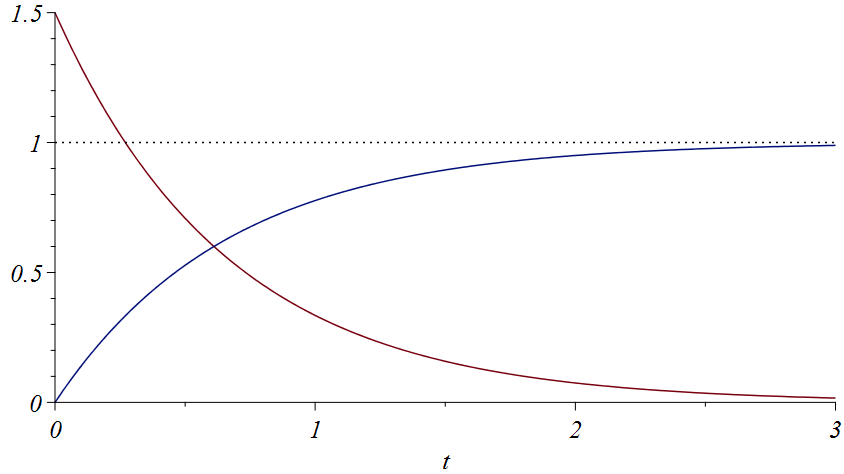
\includegraphics[width=0.7\textwidth]{images/exp-cum.png}
  \end{center}
\end{itemize}
\end{n}

\ssn{Definition}
The \emph{expected value} of a random variable $X$ with pdf $f_X(x)$ taking values in $[a,b]$ 
is given by 
 \[
    \EE(X) = \int_a^b x \, f_X(x) \dd x.
   \]  
More generally, we can take the expected value of a function $g(X)$ of our random variable $X$: 
 \[
    \EE(g(X)) = \int_a^b g(x) \, f_X(x) \dd x.
   \]
\end{n}

\ssn{Examples} 
\begin{itemize}
\item For the rod example where $f_X(x)=1/L$ on $[0,L]$, the expected value of $X$ is 
 \[
 \EE(X) =  \int_0^L  \frac1L  x \dd x = \left[ \frac{x^2}{2L}\right]_0^L = \frac{L}2, 
  \]
 which surely accords with our intuition. 
 
 Similarly (exercise)  $\EE(X^2) = L^2/3$. 
 \item 
 For the exponential distribution on $[0,\infty]$ where $f_T(t) = \lambda e^{-\lambda t}$ we have 
  \[
 \EE(T)= \int_0^\infty u \, \lambda e^{-\lambda u} \,\dd u = 
   \left[ - u e^{-\lambda u} \right]_0^\infty +
   \int_0^\infty e^{-\lambda t} \dd t = 0 + \frac1\lambda = \frac1\lambda
  \]
 where at the start we integrated by parts. 
\end{itemize}

\end{n}


\sse{} In a model of a call centre, at a given moment, the time in seconds until the next call arrives is a random variable $T$ that has a pdf of the form 
 \[
    f_T(t) =  k e^{-t/8}, \qquad \text{where $t \in [0,\infty)$ and $k$ is a constant to be determined.}
 \] 
What is the probability that a call arrives in the first four seconds? What is $\EE(T)$?   (Answers: $k=1/8$ comparing with the general exponential distribution; the expected value is thus $8$ also from the general formulae above. The integral for the probability should evaluate to approx 0.3935.) 
 \end{e}

\sse{}
The random variable $X$ defined on the interval $[0,1]$ has pdf given by $f_X(x) = k \sqrt{1-x^2}$.  Find the value for $k$ and find the expected value of $X$. No explicit integration should be necessary! 
(You should arrive at $k=2/\pi$.) 
\end{e}

\sss
Notice that the graph of $y = \sqrt{1-x^2}$ is a unit semicircle so the area under it is $\pi/2$.  Alternatively, integrate!
\end{s}


\subsection{Notes} 


\ssn{Foundations}
We will not present a completely rigorous version of the foundations of continuous probability. The fundamental difficulty is that an event will be a subset of the sample space and it needs to be a subset over which a suitable pdf can be integrated, and we do not study integration rigorously until later in the degree. 

Clearly, if we assume that $f_X(x)$ is piecewise continuous we can integrate over intervals and it does not matter if endpoints are included because the probability of a single point in the sample space is zero. It is reasonable to take finite (or even countably infinite) unions of intervals to be events since integrals add. Individual points are events, but their probability is zero and so they are not generally interesting. 

We will assume that probability functions defined by integrals obey the fundamental axioms in \S\ref{pf} and thus we assume their consequences such as \S\ref{pp} and inclusion-exclusion (\S\ref{gie}). 
\end{n}

\ssn{The Gamma function}
The \emph{Gamma function} is a way of defining factorials for all positive real numbers rather than just integers. 
We define 
 \[
    \Gamma(z) = \int_0^\infty x^{z-1} e^{-x} \dd x, \quad \text{where $z>0$}.  
 \]
Integrating by parts (where we differentiate the term $x^{z-1}$) we get 
 \begin{eqnarray*} 
  \Gamma(z)  &=& \int_0^\infty x^{z-1} e^{-x} \dd x \\
  &=& \left[ - x^{z-1} e^{-x}  \right]_0^\infty + 
    \int_0^\infty (z-1)x^{z-2} e^{-x} \dd x \\
    &=&  (z-1) \int_0^\infty x^{z-2} e^{-x} \dd x = 
     (z-1) \Gamma(z-1) 
 \end{eqnarray*} 
 Also, $\Gamma(1) = 1$ by an easy integral. So by the above, $\Gamma(2) = 1 . \Gamma(1) = 1$. And $\Gamma(3) = 2 \Gamma(2)=2$, and $\Gamma(4) = 3 \Gamma(3) = 6$. Carrying on, we see that for non-negative integers 
 \[
      \Gamma (n) = (n-1)!. 
 \]
It is annoying that the definition of the gamma function is somehow ``off by one'' compared to the factorials, but we are stuck with it.    
\end{n}

\ssn{A useful formula}
For $x, \lambda >0$ we have 
 \[
      \int_0^\infty x^{z-1} e^{-\lambda x} \dd x = \frac{1}{\lambda^z}  \Gamma(z). 
 \]
This is derived by changing variables, substituting $u=\lambda x$. 
\end{n} 

\ssn{The Gamma distribution} 
The \emph{gamma distribution} $\Gamma(\alpha, \lambda)$ where $\alpha>0$ and $\lambda >0$  is the continuous probability distribution on $[0, \infty)$ with pdf 
 \[
    f_X(x) = \frac{\lambda^\alpha}{\Gamma(\alpha)} 
     x^{\alpha -1} e^{-\lambda x}. 
 \]
Note that when $\alpha = 1$ we have the exponential distribution that we studied earlier. 

The Gamma distribution is not a ``core'' distribution for us: we will use it for some examples, but familiarity with when to use it is not expected. (But it is important: for example, the $\chi^2$ distribution used in statistics is a special case of gamma.)  
\end{n} 


\subsection{Exercises and problems}

\sse 
Invent a random variable $X$ defined on some interval $I \subseteq \RR$ that is sufficiently simple that you can compute its expected value.   
\end{e}

\sse{}
A room has two new light bulbs fitted and left permanently on at time $t=0$. They are the only illumination in the room. Each one independently has a failure time described by an exponential random variable $T$ with parameter $\lambda = 1$. 
\begin{enumerate}
    \item Write down the pdf, cdf and expected value of $T$.
    \item Consider a time $t=x$. What is the probability that both bulbs have failed (and so the room is dark) at the time $t=x$? 
    \item Let $X$ be the random variable which is the time that the room goes dark.  Compute the pdf of $X$ and its expected value. 
\end{enumerate}
(Hint: the second part is asking you to calculate the cdf of $X$.) 
\end{e}

